\documentclass{article}
\usepackage{graphicx}%
\usepackage{multirow}%
\usepackage{amsmath,amssymb,amsfonts}%
\usepackage{amsthm}%
\usepackage{mathrsfs}%
\usepackage[title]{appendix}%
\usepackage{xcolor}%
\usepackage{textcomp}%
\usepackage{manyfoot}%
\usepackage{booktabs}%
\usepackage{algorithm}%
\usepackage{algorithmicx}%
\usepackage{algpseudocode}%
\usepackage{listings}%


\providecommand{\keywords}[1]{\textbf{\textit{Keywords: ---}} #1}%keywords

\usepackage{parskip} %puts \noindent everywhere


\usepackage{caption}
\DeclareCaptionFormat{citation}{%
  \ifx\captioncitation\relax\relax\else
    \captioncitation\par
  \fi
  #1#2#3\par}
\newcommand*\setcaptioncitation[1]{\def\captioncitation{\textit{Source:}~#1}}%to add sources to figures
\let\captioncitation\relax
\captionsetup{format=citation,justification=centering}



%https://www.overleaf.com/project/642180d8a08db24a02633ac7


\usepackage{hyperref} 
% Hyperref setup
\hypersetup {
    colorlinks=true,
    urlcolor=blue
}

\usepackage{apacite}

\raggedbottom
%%\unnumbered% uncomment this for unnumbered level heads







\begin{document}

\title{\huge \scshape{Optimal TSP Solvers: Time-Constrained Algorithm Analysis}}
\author{
    \small \scshape{Harry Zhang} \\ 
    \small \scshape{Supervisors: Per-Olof Freerks and Felicia Dinnetz} \\
    \scriptsize \scshape{Kungsholmens Gymnasium}
}



\maketitle






\abstract{\noindent The abstract serves both as a general introduction to the topic and as a brief, non-technical summary of the main results and their implications. Authors are advised to check the author instructions for the journal they are submitting to for word limits and if structural elements like subheadings, citations, or equations are permitted. The codes are available at \href{https://github.com/hairez/diploma-project}{https://github.com/hairez/diploma-project}.}

\keywords{travelling salesman problem, Euclidean distance, graph, Keyword4}




\newpage

\tableofcontents

\newpage


\section{Introduction}\label{Introduction}

\subsection{Background}\label{Background}
Consider a salesman that wants to visit a number of cities around the world. The salesman does not have to visit the cities in any particular order, but after the salesman has visited all the desired cities, the salesman has to return to the city it started out in. It is fairly straightforward how to find any path that works, but what is the path with the shortest Euclidean distance$_{\ref{Euclidean distance}}$ that visits all the cities and returns to the initial starting position?
This is the problem statement of the classic problem called \textit{The travelling salesman problem}, but it is also called \textit{the travelling salesperson problem}, or just \textit{TSP} for short.


\begin{figure}[ht]
 \centering
 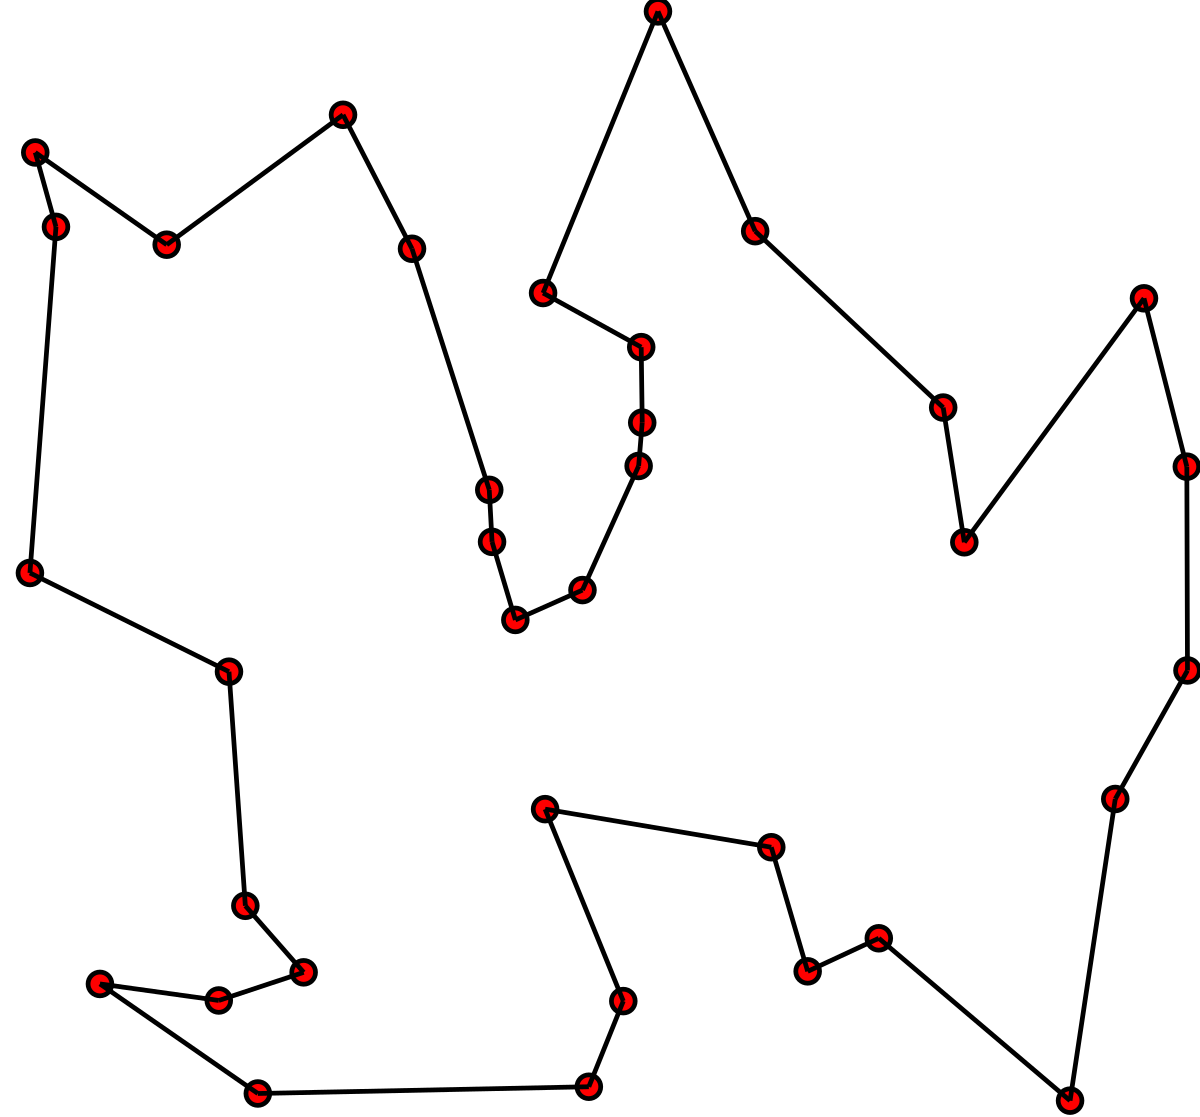
\includegraphics[scale=.15]{docs/pictures/tsp.png}
 \caption{TSP interpreted as a graph where a path is found. \cite{wiki:TSP}}
 \label{Figure:TSP-as-graph}
\end{figure}

\noindent
The travelling salesman problem could also be interpreted as a weighted undirected graph$_{\ref{undirected weighted graph}}$ with a given number of nodes. Each node is a city that the travelling salesman has to visit. The edges between each node have a specific value or length, which signifies the Euclidean distance between each pair of cities. 
\newline
Variations of the traveling salesman problem exist \cite{gutin_punnen_2007}, however, the version where the goal is to minimize the distance in Euclidean space is currently an NP-complete$_{\ref{NP-complete}}$ problem \cite{PAPADIMITRIOU1977}. 
\newline
Evidence shows that there exist no algorithms that could find the definite shortest path in polynomial time, at the same time as there are no algorithms that can guarantee any accuracy in any given map with cities. Other than that, verifying if any specific path is the most optimal is also unmanageable. \cite{PAPADIMITRIOU1977}
\newline
For example, a brute force solution could be considered to solve the classic travelling salesman problem, where all possible permutations of the order are computed, and then picking the shortest path out of all possible paths. Although this would be applicable to a smaller number of cities, the number of permutations possible would have a factorial$_{\ref{factorial}}$ growth the more cities that have to be visited. 
\newline
It is an NP-hard problem and there are a lot of different heuristic solutions. Some solutions might work better in some situations than others. In this research, different algorithms are going to be tested on different test cases within a set amount of time. The algorithms being tested in this paper are variations of the following algorithms: Dijkstra's algorithm, the Genetic algorithm with random swapping, and the Genetic algorithm with 2-opt swapping.

contextualize the topic. What could the traveling salesman problem be used for? - Robots pathfinding, efficiency. drilling holes on a plane wood plank. 
It is important to find a relatively fast approach that is both efficient in finding the most optimal path and in a short period of time, especially when a large amount of input is considered. 


\subsection{Aim}\label{Aim}
The aim of this paper is to find the limits of different heuristic algorithms for solving the travelling salesman problem. 

\subsection{Research Question}\label{RQ}
What algorithm could find the shortest path in a weighted graph, in a set amount of time?



\subsection{Theory}\label{Theory}

\subsubsection{Notations and definitions}\label{Notation and definitions}

In this section, a list of basic mathematical and computer scientific definitions and terms are explained. 
\newline

\begin{enumerate}   %use the following to refer back to this part:
                    %$_{\ref{Polynomial}}$
 
  \item \textit{The Euclidean distance} between two points $p_1=(x_1,y_1)$ and $p_2=(x_2,y_2)$ is defined as $\sqrt{(x_2-x_1)^2+(y_2-y_1)^2}$. \label{Euclidean distance}
  \item Undirected weighted graph is \label{undirected weighted graph}
  \item A problem is \textit{NP-complete} if \label{NP-complete}
  \item The \textit{factorial} of a given non-negative integer $n$ is denoted by $n!$. It is the product of all positive integers less than or equal to $n$. $$n! = n \cdot (n-1) \cdot (n-2) \cdot ... \cdot 2 \cdot 1 .$$\label{factorial}
\end{enumerate}




\subsubsection{Big O Notation}\label{Big O}
When computer scientists want to compare different kinds of algorithms, they can describe the efficiency with a mathematical function that describes the estimated run time of the algorithm using Big O notations. Big O notations is a way of describing the time complexity of an algorithm, which refers to how long an algorithm takes to complete based on the size of its input. The big O notations show a huge difference when comparing the worst-case scenarios for each algorithm.
\newline
 The "O" in Big O notation stands for "order of magnitude", which means that the function described grows a the same rate or within a constant factor as the function that is given. Hence when describing time complexities using big O notations, the coefficient becomes irrelevant. For example, an algorithm such as calculating the roots of a quadratic equation takes a constant time regardless of the input size and has a time complexity of $O(1)$, even though the algorithm could possibly perform more than $1$ operation. If the time complexity of an algorithm grows linearly with the size of the input, the time complexity of the algorithm would be $O(n)$. An example of an algorithm with this time complexity would be to calculate the sum of an array with $n$ integers since it is required to iterate through the whole array, as long as no other sum using this array has been pre-computed. Some other examples common time complexities are: $O(\log{n})$, $O(n \log{n})$, $O(n^2)$, $O(2^n)$, and $O(n!)$.


\newline

\subsubsection{Random Algorithm}\label{Dijkstras}
generate a random path, and calculate the length. repeat.
The random algorithms generate a random permutation and calculate the length of the path generated. It always stores the path with the shortest path and repeats this algorithm until the time limit is reached. This algorithm has a time complexity of $O(n)$, since the generation of a random path has to iterate through each possible node. 

\begin{algorithm}
\caption{Algorithm that generates random paths}\label{Random Algorithm}
\begin{algorithmic}

\While{Less than 2 seconds has passed}
\State $order \gets $ random permutation of the $n$ nodes
\State $currPath \gets calculatePath(order)$
\If{$bestPath > currPath$}
\State $bestOrder \gets order$
\State $bestPath \gets currPath$
\EndIf
\EndWhile

\end{algorithmic}
\end{algorithm}


\subsubsection{Dijkstra's Algorithm}\label{Dijkstras}
Dijkstra's algorithm is 
originally a $O(n^2)$ algorithm. however, by only comparing the log2(n) random neighbors, it would become $O(nlog(n))$


\subsubsection{Genetic Algorithm with Random Swapping}\label{Random Swapping}
algorithm that requires $O(n)$. however for each swap, it takes $O(1)$. run until 2 seconds has gone by.

\subsubsection{Genetic Algorithm with 2-opt swapping}\label{2-opt swapping}
algorithm that requires $O(n)$. however for each swap, it takes $O(1)$. run until 2 seconds has gone by.


\subsubsection{Generation of Maps}\label{subsubsec1}
How does each map get generated?

map4 Sweden: https://github.com/sphrak/svenska-stader/blob/master/src/svenska-stader.csv  took the top 1000 or 10000 most populated cities in sweden

map5: USA: https://simplemaps.com/data/us-cities. took the top populated 1000 or 10000 most populated cities in USA.


\subsubsection{Integers vs floats}\label{subsubsec1}
Integers and floats are two common data types for numbers. Integers are used to store whole numbers, while floats are used to store decimal numerals. Computers are known to be very inefficient when it comes to handling float numbers.
this is why all coordinates of the maps are integers, even though coordinates on a real map are not necessarily integers. 




\section{Method}\label{sec2}
Use different algorithms to solve the TSP in different maps (weighted undirected graphs).




Dependent: The length of the path
Independent: the algorithm


Constant variables: The maps and the max amount of time. Programming language: python

The maps: 

\subsection{Limitations}\label{subsec3}







\section{Results}\label{sec3}

Sample body text. Sample body text. Sample body text. Sample body text. Sample body text. Sample body text. Sample body text. Sample body text.

show table






\section{Discussion}\label{sec4}


\subsection{Generalised result}\label{subsec1}
which algorithm showed the best results overall?


\subsection{Specified }\label{subsec2}
what algorithm could be good in what situation?


\subsection{Evaluation and further research}\label{subsec3}
using $O(n^2)$ algorithms such as 
greedy algorithm
Christofides algorithm
Simulated annealing.
3 opt. or even Lin-Kernighan Heuristic algorithm
Longer time-constraints?
combination of these? For example start with a greedy solution, and then improve it by applying 3-opt.

\section{Conclusion}\label{sec5}






\newpage
\bibliographystyle{apacite}
\bibliography{references.bib} \label{sec6}



\end{document}
